\documentclass[xcolor=dvipsnames, 9pt]{beamer}

\usepackage{amssymb}
\usepackage{amsfonts}
\usepackage{amsmath}
\usepackage{hyperref}
\usepackage{natbib}
\usepackage{color}
\usepackage{pdfsync}
\usepackage{chancery}
\usepackage{movie15}
\usepackage{pgfpages}
\usepackage{fancyvrb}
\usepackage{colortbl}
\usepackage{multirow}

\usepackage{graphicx}
\graphicspath{{../images/figures/}{../images/logos/}{../images/graphs}/}

\usepackage{beamerthemesplit}
\usetheme{Copenhagen}
\definecolor{title}{RGB}{128,148,182}
\usecolortheme[named=title]{structure} 
\setbeamertemplate{navigation symbols}{}
\setbeamertemplate{itemize items}[triangle]
\setbeamertemplate{enumerate items}[default]
\setbeamertemplate{footline}[page number]{}
%\setbeameroption{show notes on second screen}
% \logo{
\includegraphics[width = 2cm]{../images/logos/500px-NYU_logo.png}}

%\usepackage{listings,bera}
\usepackage{listings,arev}
\definecolor{keywords}{RGB}{128,148,182}
\definecolor{comments}{RGB}{60,179,113}
\lstset{language=Python,
        numbers=left,
        showstringspaces=false,
        numberstyle=\tiny,
        frame=leftline,
  keywordstyle=\color{keywords}\bfseries,
  commentstyle=\color{YellowOrange}\emph
}

\newenvironment{code}{\begin{semiverbatim} \begin{footnotesize}}
{\end{footnotesize}\end{semiverbatim}}


\newcommand{\R}{\mathbb{R}}
\renewcommand{\d}{\mathsf{d}}
\newcommand{\dd}{\partial}
\newcommand{\E}{\mathsf{E}}
\newcommand{\bb}{\mathbf}



\title{1 - Introduction to NetworkX}
\author{Drew Conway and Aric Hagberg}
%\institute{
\includegraphics[width = 4cm]{500px-NYU_logo.png}}
\date{June 29, 2010}

\begin{document}
\begin{frame}[plain]
\titlepage
\end{frame}

\begin{frame}
\frametitle{Networks}

Vast amounts of data are being generated and collected

\begin{itemize}
\item Sociology: WWW, email, social networking  
\item Technology: Internet, telecommunications, power grid
\item Biology: protein interactions, genetic regulatory networks, epidemiology
\end{itemize}

\begin{columns}[c]
\begin{column}{0.33\textwidth}
\centerline{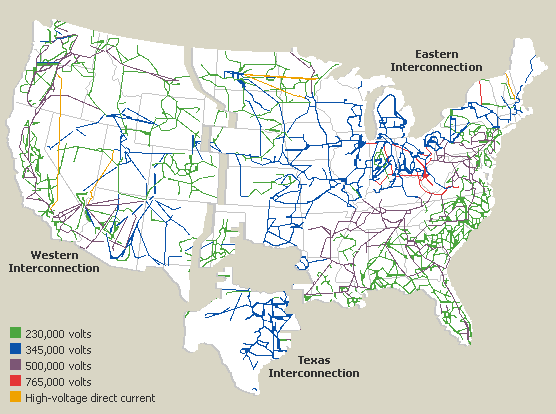
\includegraphics[width=1.0\columnwidth]{powergrid}}
\end{column}
\begin{column}{0.33\textwidth}
\centerline{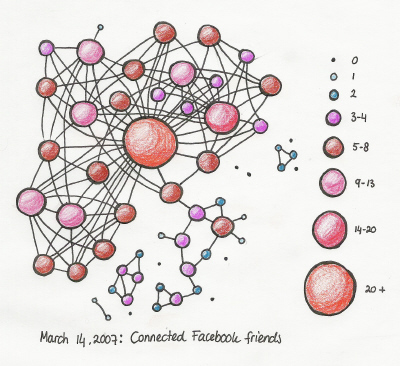
\includegraphics[width=1.0\columnwidth]{smallgraph}}
\end{column}
\begin{column}{0.33\textwidth}
\centerline{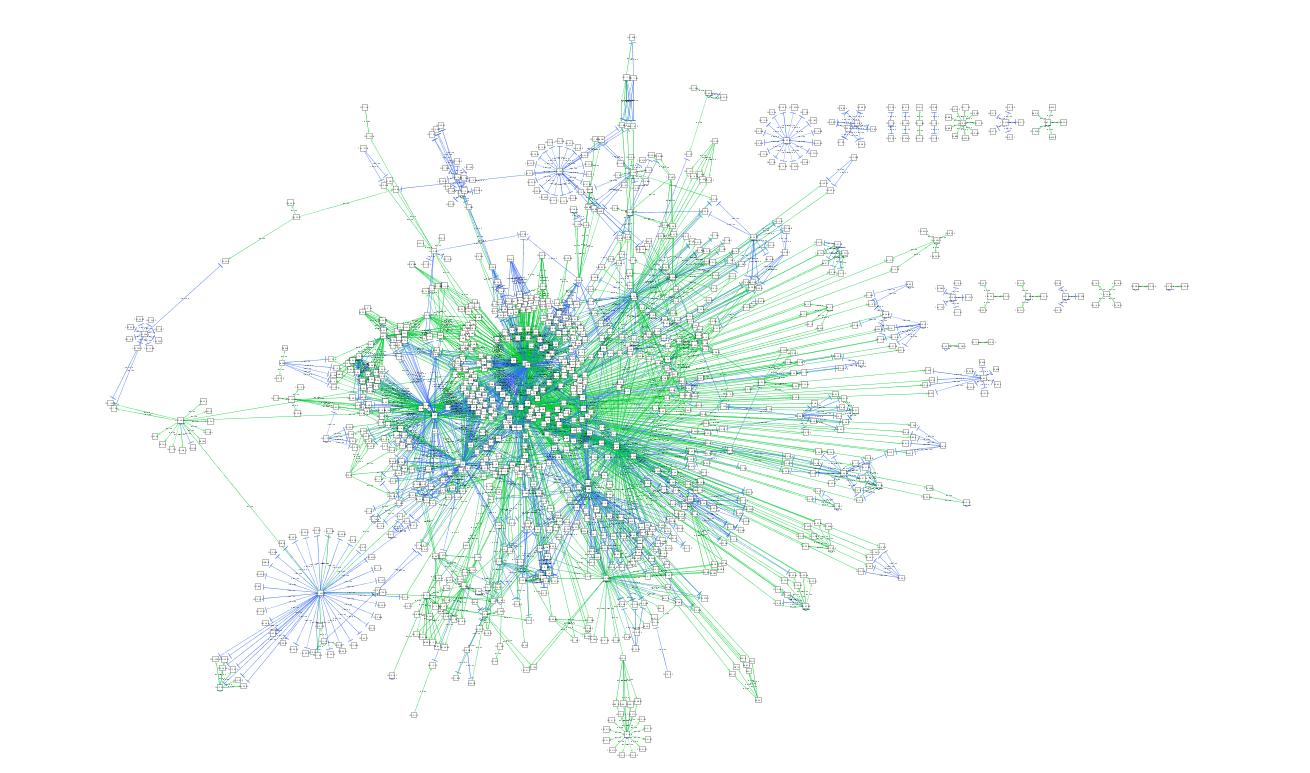
\includegraphics[width=1.0\columnwidth]{ecoli}}
\end{column}
\end{columns}

\bigskip
Need theory, analysis, models 
%FIXME: new slide?  reference earlier talks?

\end{frame}

% start with examples on motivation 
\begin{frame}
\frametitle{Example: social networks and epidemics}
Understand epidemic outbreak of diseases through modeling

Build social networks from detailed census data 

Run dynamic models for smallpox, SARS, flu, etc. 

\begin{columns}[c]
\begin{column}{0.65\textwidth}
\centerline{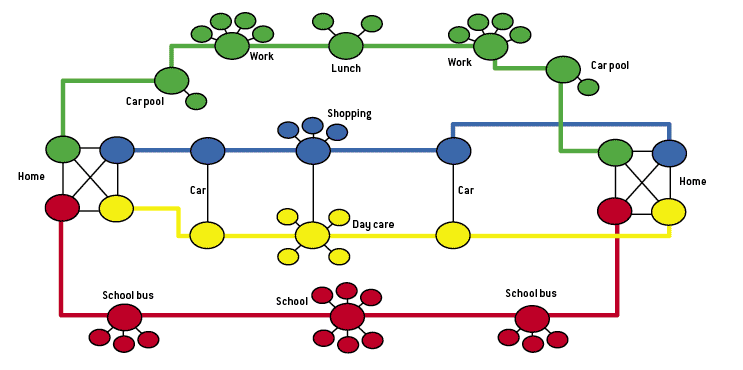
\includegraphics[width=1.0\columnwidth]{socialnet}}
\centerline{\small Building a social network}
\end{column}
\begin{column}{0.35\textwidth}

\centerline{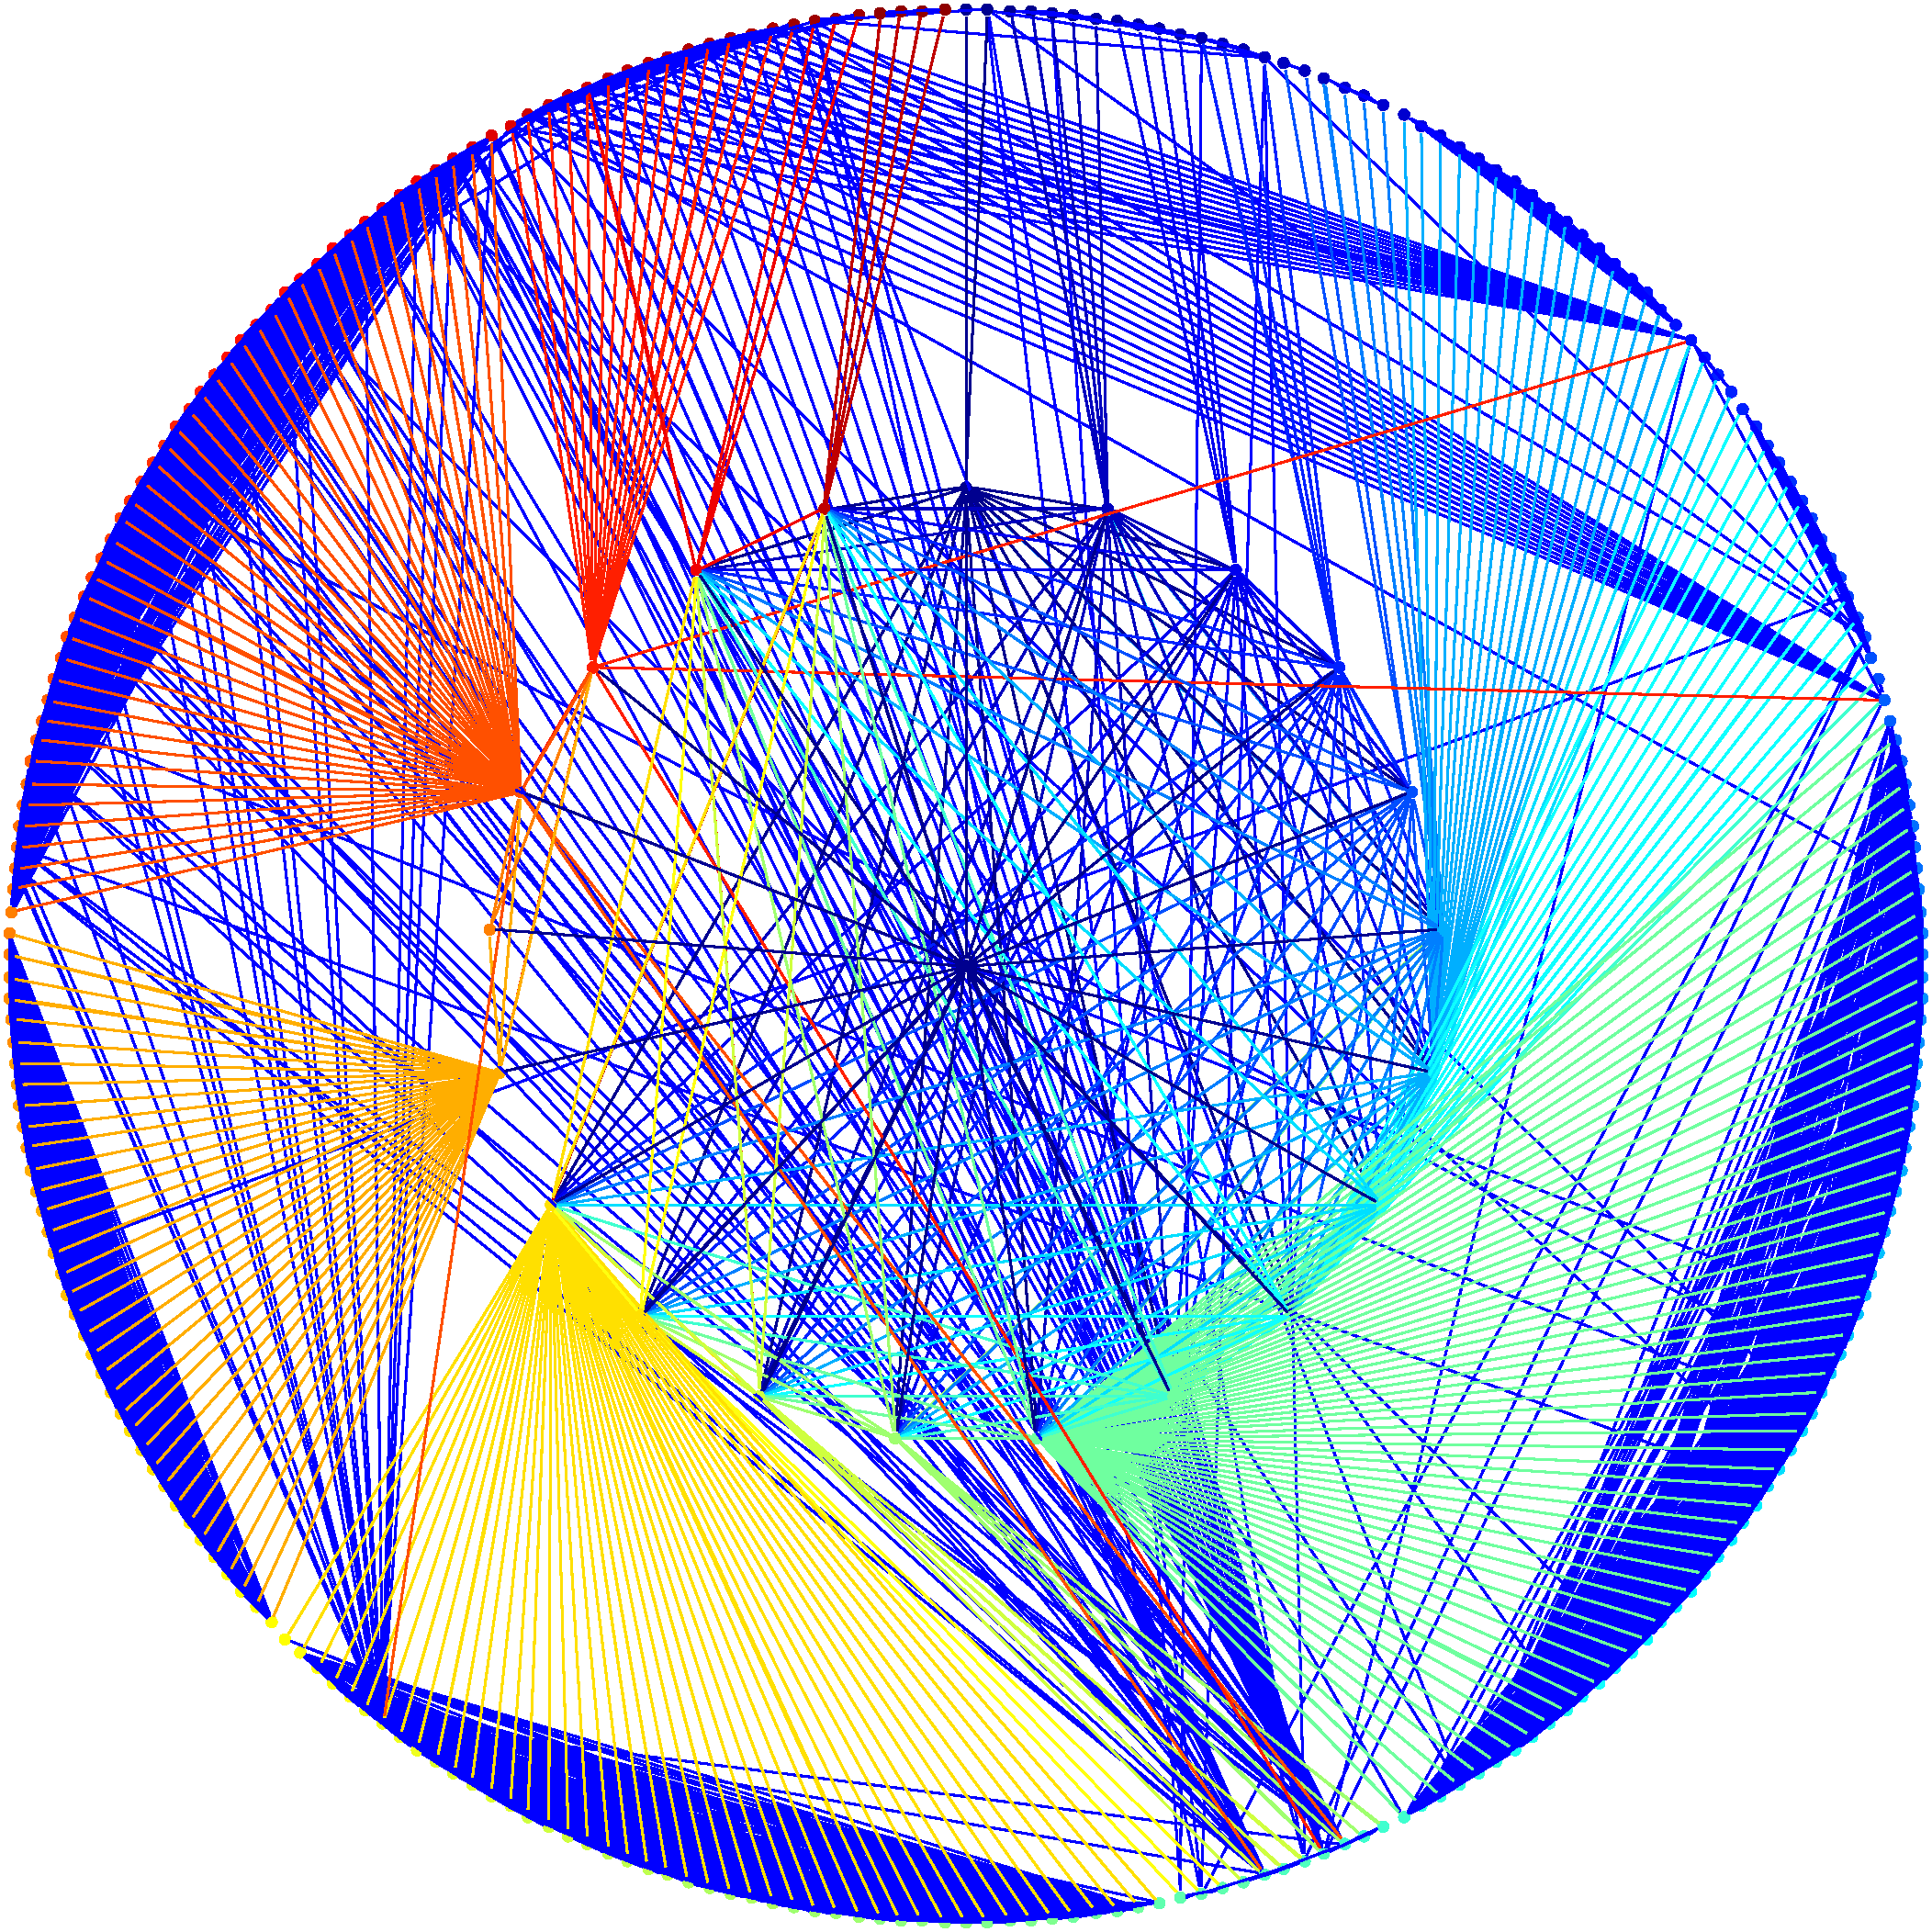
\includegraphics[width=1.0\columnwidth]{1311774-2c}}
\centerline{\small Social network of one person}
\end{column}
\end{columns}

Goal: find a good intervention strategy

\footnotesize
NISAC: EpiSimS
\end{frame}


\begin{frame}
\frametitle{Example: interdiction}
Problem: smuggling of nuclear material in transportation network
\begin{columns}
\begin{column}{0.5\textwidth}
\centerline{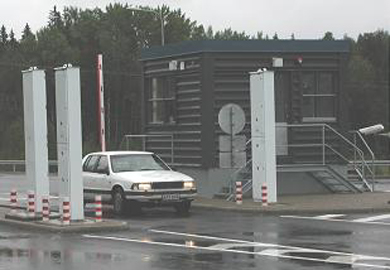
\includegraphics[width=1.0\columnwidth]{NTI_car_border}}
\centerline{\small Detector at border crossing}
\end{column}
\begin{column}{0.5\textwidth}
\centerline{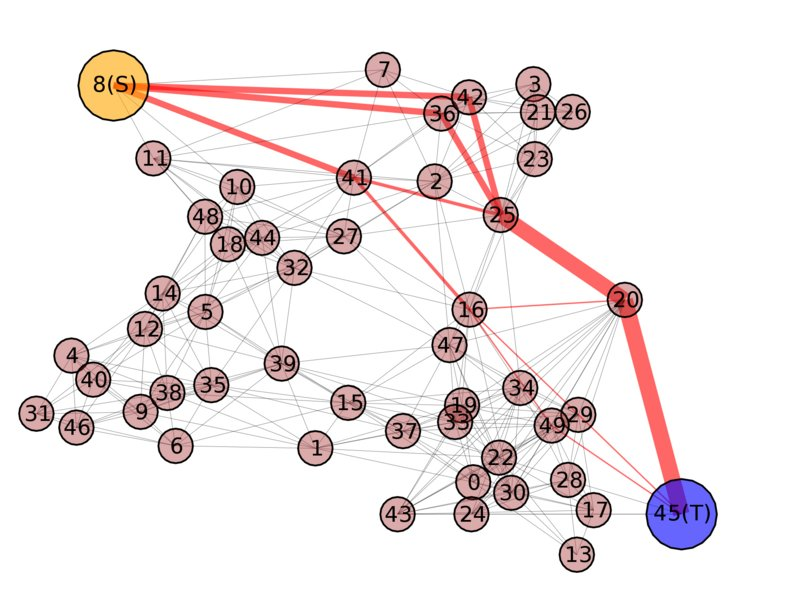
\includegraphics[width=0.95\columnwidth]{evader50newsmall}}
Find best set of roads (edges) to monitor (cut) with limited budget
\end{column}
\end{columns}
\end{frame}


\begin{frame}
\frametitle{Example: journal usage network}

\centerline{
\includegraphics[width=0.18\columnwidth]{mesur_logo}}

\bigskip

University libraries, journals, and aggregators collect 
journal usage data through web portals 

MESUR project is analyzing about 1 billion usage events

Build network from user click streams

\begin{itemize}
\item Do scholars read and cite journals in the same way?
\item Can new trends in research (new field, interdisciplinary) be
  spotted?
\item Which journals are most important according to usage?
\end{itemize}

Johan Bollen, Los Alamos

\end{frame}


\begin{frame}
\frametitle{Example: journal usage network}

\centerline{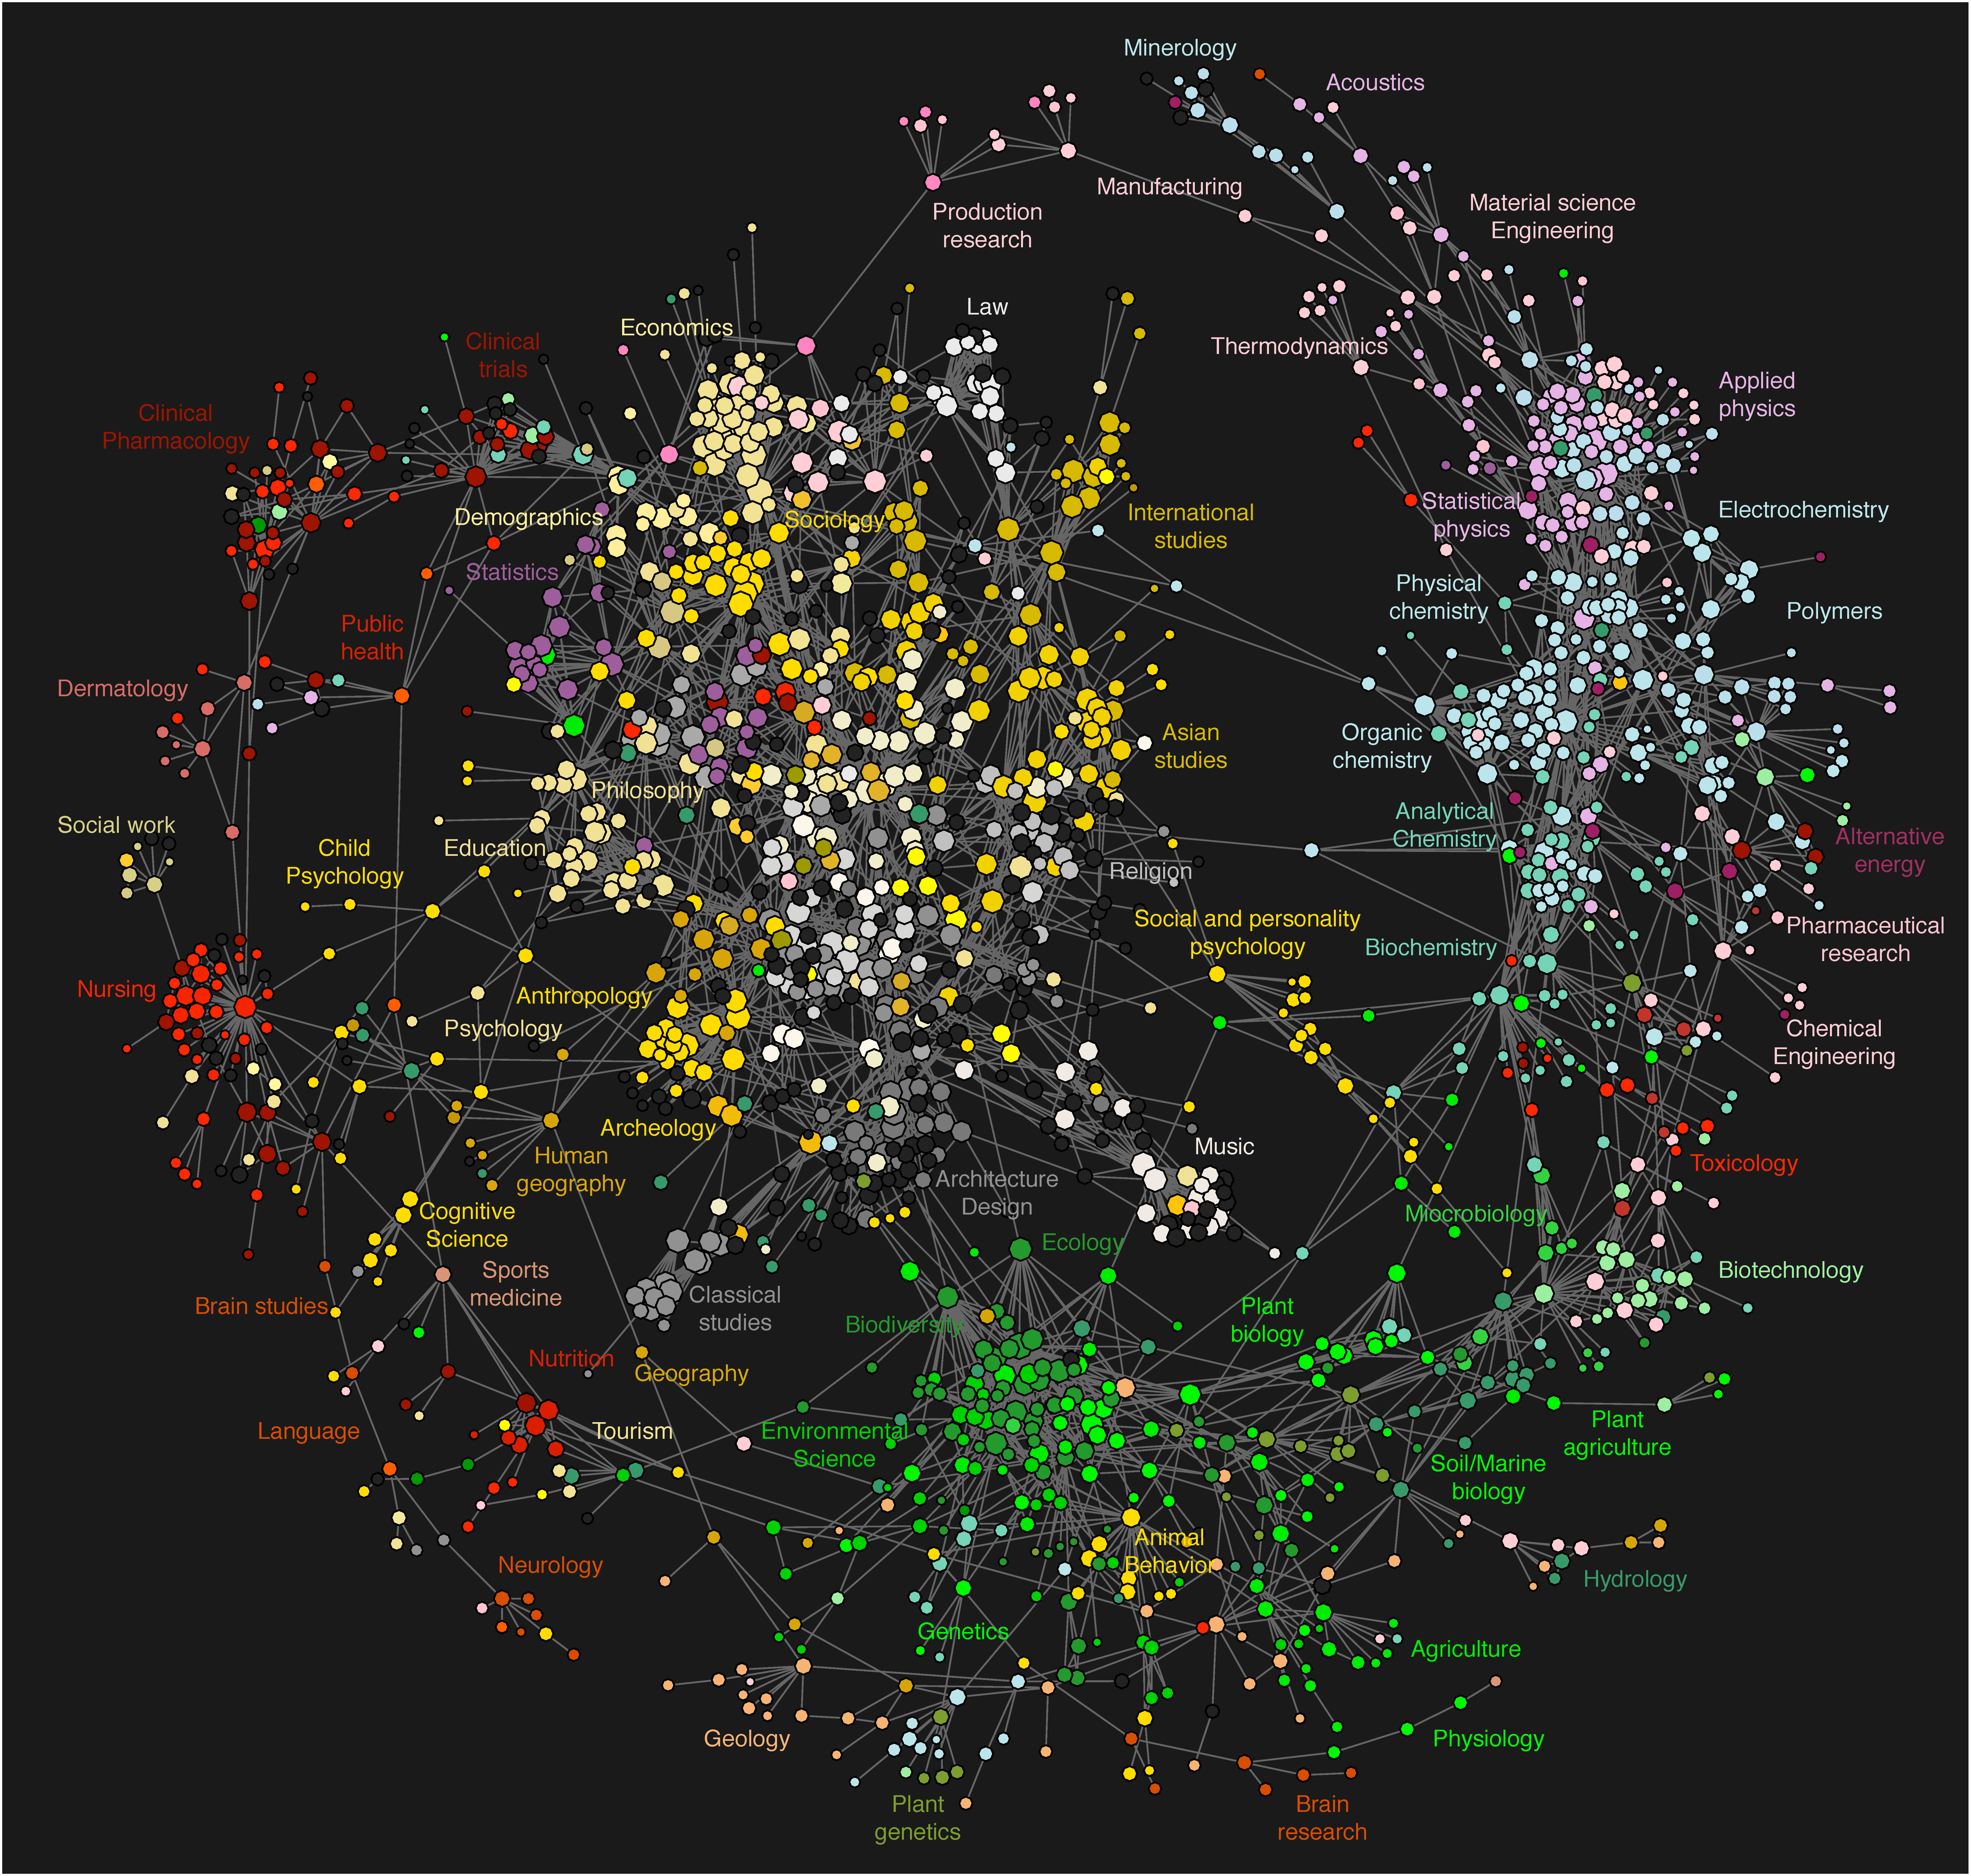
\includegraphics[width=0.8\columnwidth]{msr_all_50000red_aat_e_nolabels}}

\end{frame}

\begin{frame}
\frametitle{NetworkX project: goals and features}
\centerline{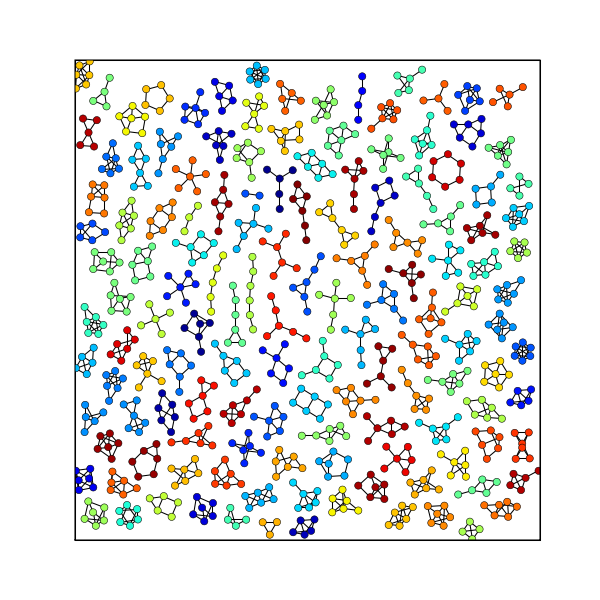
\includegraphics[width=0.8\columnwidth]{atlas}}


\end{frame}


\begin{frame}
\frametitle{Goals: Why we started project}
\begin{block}
{We needed:}
\begin{itemize}
\item Tool to study the structure and
dynamics of social, biological, and infrastructure networks
\item Ease-of-use and rapid
development in a collaborative, multidisciplinary environment 
\item Open-source tool base that can easily
grow in a multidisciplinary environment with non-expert users and developers
\item An easy interface to 
existing code bases written in C, C++, and FORTRAN 
\item To painlessly slurp in large nonstandard data sets 
\end{itemize}
\end{block}
\begin{itemize}
\item No existing API or graph implementation that was suitable 
\item Inspired by Guido van Rossum's 1998 Python graph representation essay 
\item First public release in April 2005
\end{itemize}
\end{frame}


\begin{frame}
\frametitle{Also: Fun}
\centerline{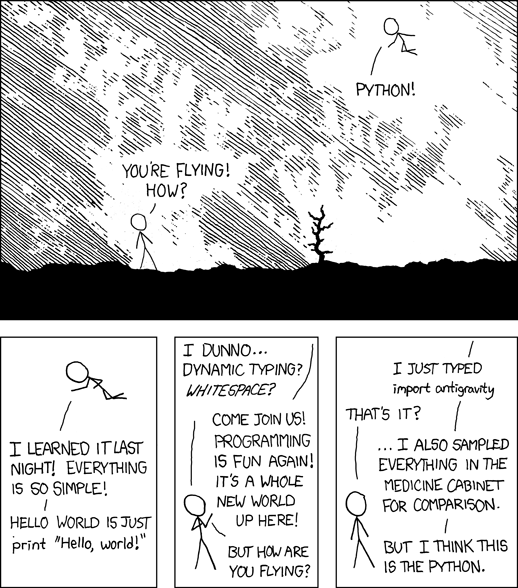
\includegraphics[width=0.65\columnwidth]{xkcd-python}}
\end{frame}




% start with examples on motivation 
\begin{frame}
\frametitle{Features: NetworkX in one slide}
\begin{columns}[c]
\begin{column}{0.65\textwidth}
\begin{itemize}
\item  Python language package for exploration and analysis of
networks and network algorithms  
\item Data structures for representing many types of networks, or graphs,
(simple graphs, directed graphs, and graphs with parallel edges and
  self loops)
\item Nodes can be any (hashable) Python object
\item Edges can contain arbitrary data
\item Flexibility ideal for representing networks found
in many different fields
\item Many unit and functional tests 
\item Online up-to-date documentation
\end{itemize}
\end{column}
\begin{column}{0.35\textwidth}
\centerline{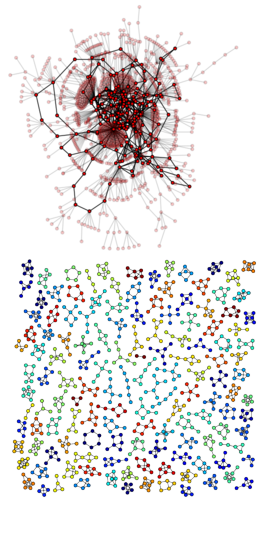
\includegraphics[width=1.0\columnwidth]{art_white}}
\end{column}
\end{columns}
\end{frame}

\begin{frame}[fragile]
\frametitle{Design decisions}

\begin{block}
{NetworkX defines no custom node objects or edge objects}

\begin{itemize}
\item ``node-centric'' view of network

\item Nodes: whatever you put in (hashable)

\item Edges: tuples with optional edge data (stored in dictionary)

\item Edge data is arbitrary and users can define custom node types

\end{itemize}
\end{block}

%% \end{frame}

%% \begin{frame}[fragile]
%% \frametitle{Design decisions}


\begin{block}
{NetworkX is all Python}
(Other projects use custom compiled code and Python: Boost Graph,
  igraph, Graphviz)

\begin{itemize}
\item Focus on computational network modeling not software tool development

\item Move fast to design new algorithms or models 

%\item Might leverage Cython or other extensions

\end{itemize}
\end{block}


\end{frame}



\begin{frame}[fragile]
\frametitle{Feature: Simple use, adding nodes}

Start Python

Import NetworkX using ``nx'' as a short name
\begin{block}{}
\begin{verbatim}
>>> import networkx as nx 
\end{verbatim}
\end{block}
The basic $Graph$ class is used to hold the network information.
Nodes can be added as follows:
\begin{block}{}
\begin{verbatim}
>>> G=nx.Graph()
>>> G.add_node(1) # integer
>>> G.add_node('a') # string
>>> print G.nodes()
['a', 1]
\end{verbatim}
\end{block}

\end{frame}


\begin{frame}[fragile]
\frametitle{Feature: nodes can be ``anything''}

Nodes can be any hashable object such as strings,
numbers, files, functions, and more
\begin{block}{}
\begin{verbatim}
>>> import math
>>> G.add_node(math.cos) # cosine function
>>> fh=open('tmp.txt','w') 
>>> G.add_node(fh) # file handle
>>> print G.nodes()
[<built-in function cos>, 
<open file 'tmp.txt', mode 'w' at 0x30dc38>]
\end{verbatim}
\end{block}


\end{frame}



\begin{frame}[fragile]
\frametitle{Feature: edges are just pairs of nodes}
Edges, or links, between nodes are represented as tuples of nodes.  
They can be added simply
\begin{block}{}
\begin{verbatim}
>>> G.add_edge(1,'a')
>>> G.add_edge('b',math.cos)
>>> print G.edges()
[('b', <built-in function cos>), ('a', 1)]
\end{verbatim}
\end{block}

If the nodes do not already exist they are automatically added to the graph.

% FIXME add picture?


\end{frame}



\begin{frame}[fragile]
\frametitle{Feature: Edge can hold arbitrary data}

\begin{columns}[T]

\begin{column}{0.7\textwidth}
Any Python object is allowed as edge data 

(e.g. number, string, image, file, ip address)

Edge data assigned and stored in a Python dictionary (default empty).

\bigskip
Use Dijkstra's algorithm to find the shortest path:

\end{column}

\begin{column}{0.3\textwidth}
\centerline{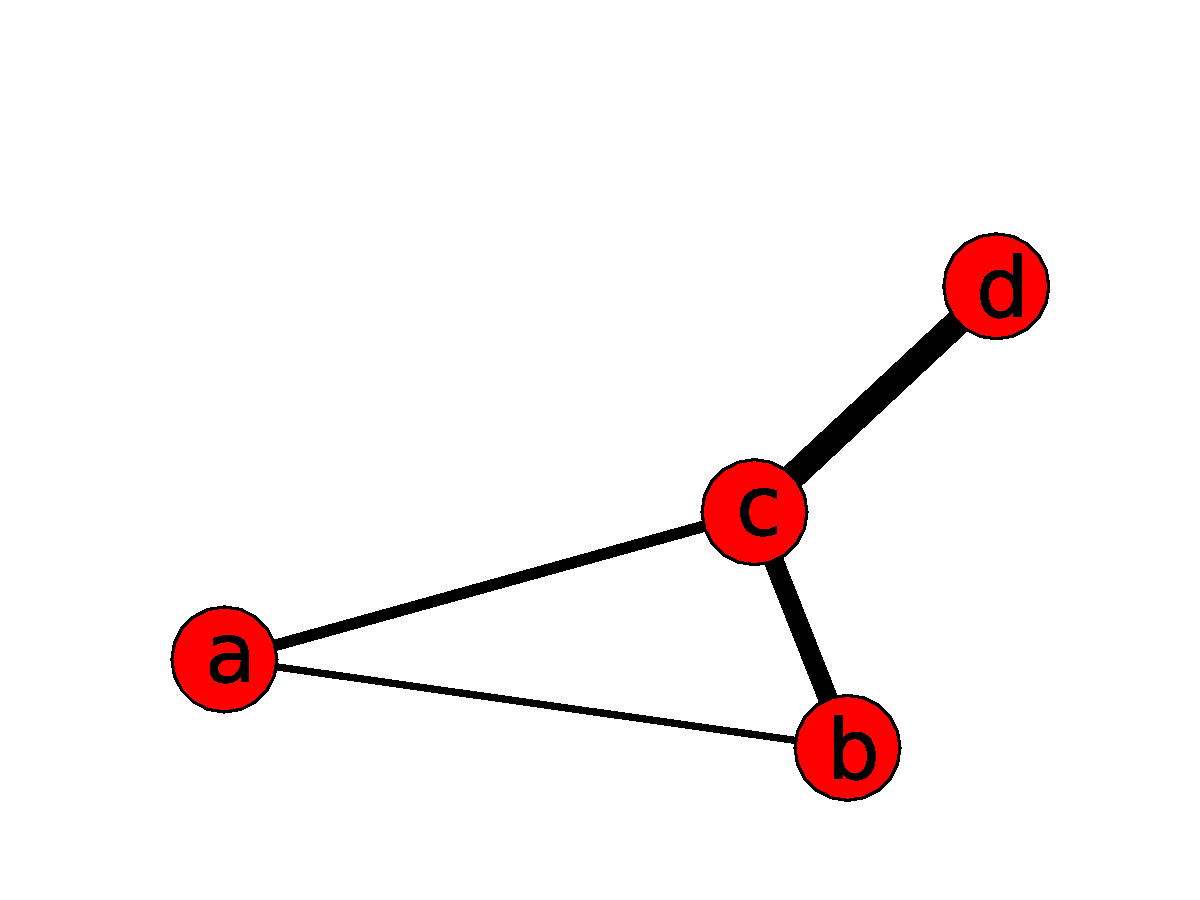
\includegraphics[width=1.5\columnwidth]{dijkstra}}
\end{column}
\end{columns}

\begin{block}{}
\begin{verbatim}
>>> G=nx.Graph()
>>> G.add_edge('a','b',weight=0.3)
>>> G.add_edge('b','c',weight=0.5)
>>> G.add_edge('a','c',weight=2.0)
>>> G.add_edge('c','d',weight=1.0)
>>> print nx.shortest_path(G,'a','d')
['a', 'c', 'd']
>>> print nx.shortest_path(G,'a','d',weighted=True)
['a', 'b', 'c', 'd']
\end{verbatim}
\end{block}

\end{frame}



\begin{frame}[fragile]
\frametitle{Feature: testing}
NetworkX has many tests that can be run by users
\footnotesize
\begin{block}{}
\begin{verbatim}
>>> import networkx
>>> networkx.test(verbosity=2)
...
Doctest: networkx.utils ... ok
Conversion from digraph to array to digraph. ... ok
Conversion from digraph to matrix to digraph. ... ok
Conversion from graph to array to graph. ... ok
Conversion from graph to matrix to graph. ... ok
Conversion from weighted digraph to array to weighted digraph. ... ok
...
Conversion from non-square array. ... ok
Conversion from digraph to sparse matrix to digraph. ... ok
Conversion from graph to sparse matrix to graph. ... ok
Conversion from weighted digraph to sparse matrix to weighted digraph. ... ok
Conversion from weighted graph to sparse matrix to weighted graph. ... ok
Conversion from graph to sparse matrix to graph with nodelist. ... ok
Conversion from non-square sparse array. ... ok
Doctest: networkx ... ok

----------------------------------------------------------------------
Ran 855 tests in 4.334s

OK
\end{verbatim}
\end{block}
\end{frame}

\begin{frame}
\frametitle{Feature: Online, up-to-date documentation}
\begin{columns}[T]
\begin{column}{0.5\textwidth}
\centerline{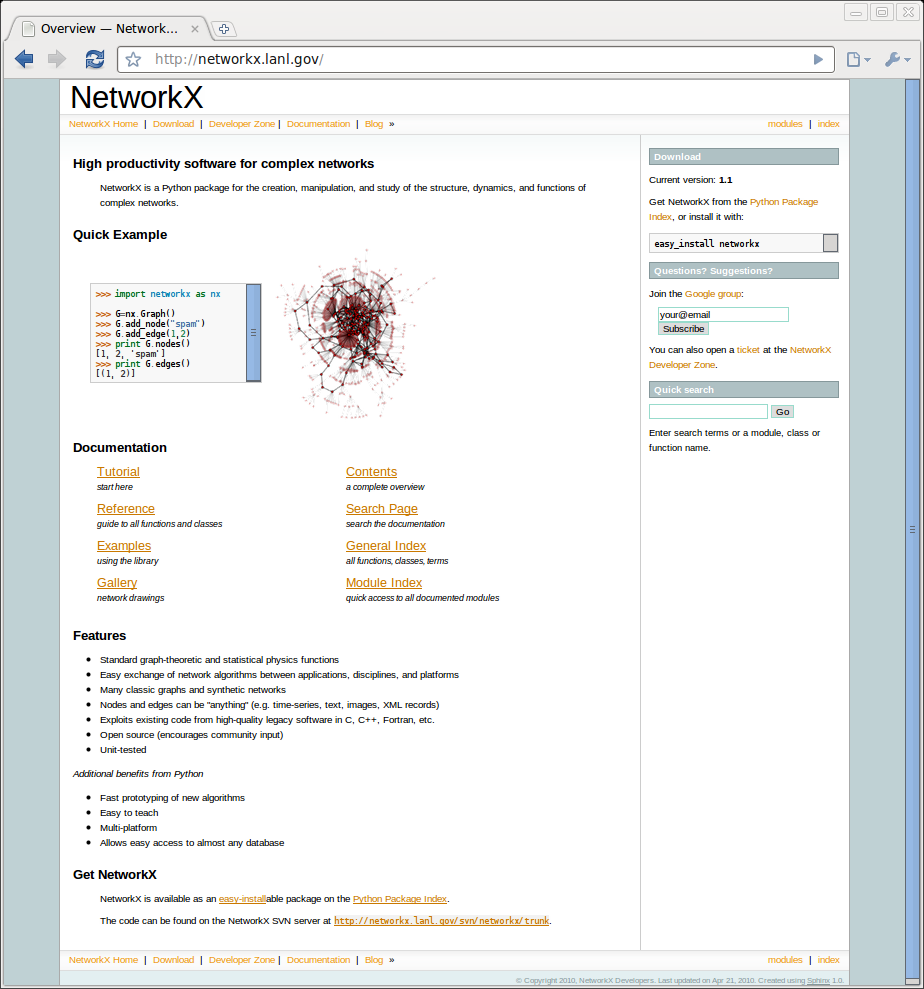
\includegraphics[width=1.0\columnwidth]{networkx-home}}
\end{column}
\begin{column}{0.5\textwidth}
\centerline{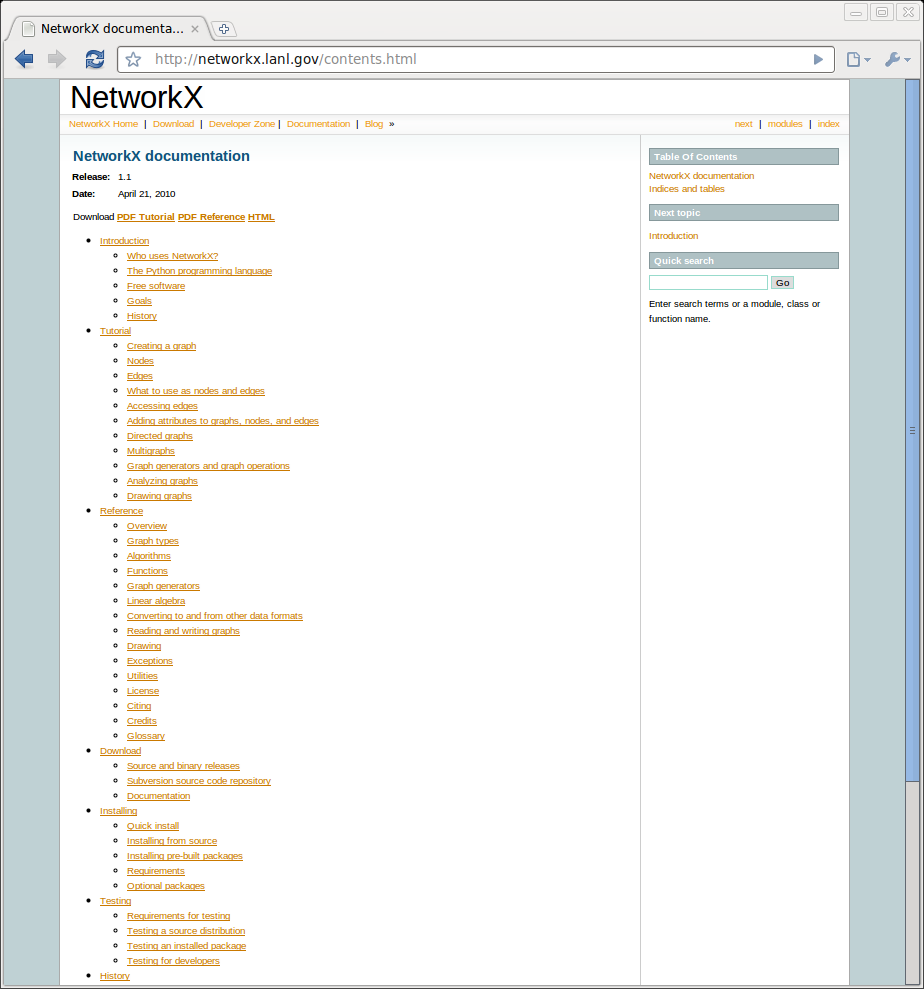
\includegraphics[width=1.0\columnwidth]{networkx-doc}}
\end{column}
\end{columns}
\end{frame}


% \begin{frame}

% Inside NetworkX

% \end{frame}


% \begin{frame}[fragile]
% \frametitle{Inside NetworkX}

% It's ``Python all the way down''

% NetworkX uses a ``dictionary of dictionaries''

% Good for adjacency list representation (sparse graphs)

% \begin{itemize}
%   \item Node $n$ is a key in the $G.adj$ dictionary 
%   \item Data is a dictionary with neighbors as keys and data $1$
% \end{itemize}

% Representation of an undirected graph with the edges $A-B$, $B-C$
% \begin{block}{}
% \begin{verbatim}
% >>> G=nx.Graph()
% >>> G.add_edge('A','B')
% >>> G.add_edge('B','C')
% >>> print G.adj
% {'A': {'B': 1}, 
%  'B': {'A': 1, 'C': 1}, 
%  'C': {'B': 1}}
% \end{verbatim}
% \end{block}
% \end{frame}

% \begin{frame}[fragile]
% \frametitle{Dictionary of dictionaries}

% Guido van Rossum proposed a dictionary of lists 

% Allows the natural expressions (Eppstein)

% \begin{itemize}
%     \item ``{\tt n in G}'' to test if the graph $G$ contains node $n$ 
%     \item ``{\tt for n in G}'' to loop over all nodes
% \end{itemize}

% Advantages of ``dict of dict'' data structure
  
% \begin{itemize}
%   \item Find edges and remove edges with two dictionary look-ups 
%   \item Prefer to ``sets'' since data can be attached to edge
%     \begin{itemize}
%       \item $G[u][v]$ returns the edge object
%     \end{itemize}
% \end{itemize}

% \footnotesize

% \begin{itemize}
% \item
% Guido van Rossum.
% Python {P}atterns - {I}mplementing {G}raphs, 1998.
% \url{http://www.python.org/doc/essays/graphs/}

% \item
% David Eppstein.
% {PADS}, a library of {P}ython {A}lgorithms and {D}ata {S}tructures,
%   2008.
% \url{http://www.ics.uci.edu/\~eppstein/PADS/}
% \end{itemize}

% \end{frame}


% FIXME ``Expressing yourself with NetworkX''

\begin{frame}[fragile]
\frametitle{Feature: Python expressivity - a simple algorithm}
Python is easy to write and read
\begin{block}{Breadth First Search}
\begin{verbatim}
from collections import deque

def breadth_first_search(g, source):
    queue = deque([(None, source)])
    enqueued =  set([source])
    while queue:
        parent, n = queue.popleft()
        yield parent, n
        new = set(g[n]) - enqueued
        enqueued |= new
        queue.extend([(n, child) for child in new])
\end{verbatim}
\end{block}
Credit: Matteo Dell'Amico
\end{frame}



% \begin{frame}[fragile]
% \frametitle{Writing a simple algorithm}
% \begin{block}{Shortest path}
% \begin{verbatim}

% def shortest_path(g, source, target):
%     paths = {None: []}
%     for parent, child in bfs(g, source):
%         paths[child] = paths[parent] + [child]
%         if child == target:
%             return paths[child]
%     return None # or raise appropriate exception 

% \end{verbatim}
% \end{block}
% Credit: Matteo Dell'Amico
% \end{frame}


\begin{frame}[fragile]
\frametitle{Feature: Compact code - building new generators}
\centerline{
\includegraphics[width=0.7\columnwidth]{model_title}}
\centerline{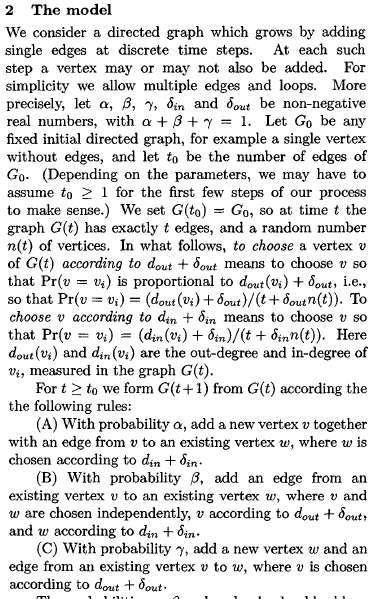
\includegraphics[width=0.4\columnwidth]{model}}
\end{frame}

\begin{frame}[fragile]
\frametitle{Feature: Compact code - building new generators}
\begin{block}{}
\tiny
\begin{verbatim}
import bisect
import random
from networkx import MultiDiGraph

def scale_free_graph(n, alpha=0.41,beta=0.54,delta_in=0.2,delta_out=0):
    def _choose_node(G,distribution,delta):
        cumsum=0.0
        psum=float(sum(distribution.values()))+float(delta)*len(distribution)
        r=random.random()
        for i in range(0,len(distribution)):
            cumsum+=(distribution[i]+delta)/psum
            if r < cumsum:  
                break
        return i

    G=MultiDiGraph()
    G.add_edges_from([(0,1),(1,2),(2,0)])
    gamma=1-alpha-beta

    while len(G)<n:
        r = random.random()
        if r < alpha:
            v = len(G) 
            w = _choose_node(G, G.in_degree(with_labels=True),delta_in)
        elif r < alpha+beta:
            v = _choose_node(G, G.out_degree(with_labels=True),delta_out)
            w = _choose_node(G, G.in_degree(with_labels=True),delta_in)
        else:
            v = _choose_node(G, G.out_degree(with_labels=True),delta_out)
            w = len(G) 
        G.add_edge(v,w)
    return G

\end{verbatim}
\end{block}
\end{frame}

\begin{frame}[fragile]

\frametitle{Feature: leveraging libraries}

Use well-tested numerical and statistical libraries 

E.g. convert Graphs to and from  NumPy (and SciPy sparse) matrices 

Example: Find eigenvalue spectrum of the graph Laplacian

\begin{columns}[T]
\begin{column}{0.75\textwidth}

\begin{block}{}
\begin{verbatim}
>>> L=nx.laplacian(G)  
>>> print L  # a NumPy matrix
[[ 1. -1.  0.  0.  0.  0.]
 [-1.  2. -1.  0.  0.  0.]
 [ 0. -1.  2. -1.  0.  0.]
 [ 0.  0. -1.  2. -1.  0.]
 [ 0.  0.  0. -1.  2. -1.]
 [ 0.  0.  0.  0. -1.  1.]]
>>> import numpy.linalg
>>> print numpy.linalg.eigvals(L)
[  3.7321e+00   3.0000e+00   2.0000e+00
   1.0000e+00  -4.0235e-17   2.6795e-01]
\end{verbatim}
\end{block}
\end{column}
\begin{column}{0.2\textwidth}
\centerline{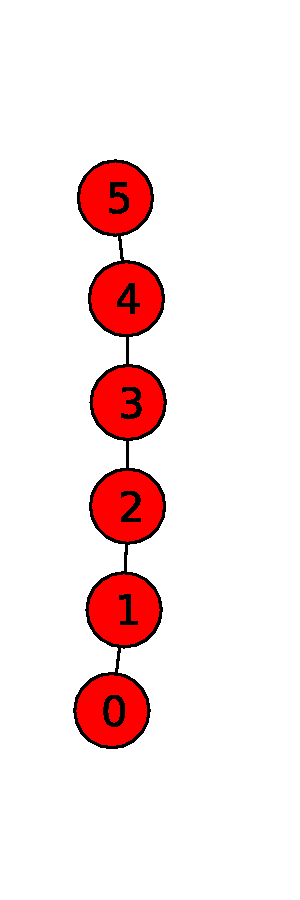
\includegraphics[width=1.0\columnwidth]{path6}}
\end{column}

\end{columns}

\end{frame}

\begin{frame}[fragile]
\frametitle{Feature: drawing}

Built-in interface to Matplotlib plotting package 

Node positioning algorithms based on force-directed, spectral, and geometric methods

\begin{block}{}
\begin{verbatim}
>>> G = nx.circular_ladder_graph(12)
>>> nx.draw(G) # Matplotlib under the hood
\end{verbatim}
\end{block}
\centerline{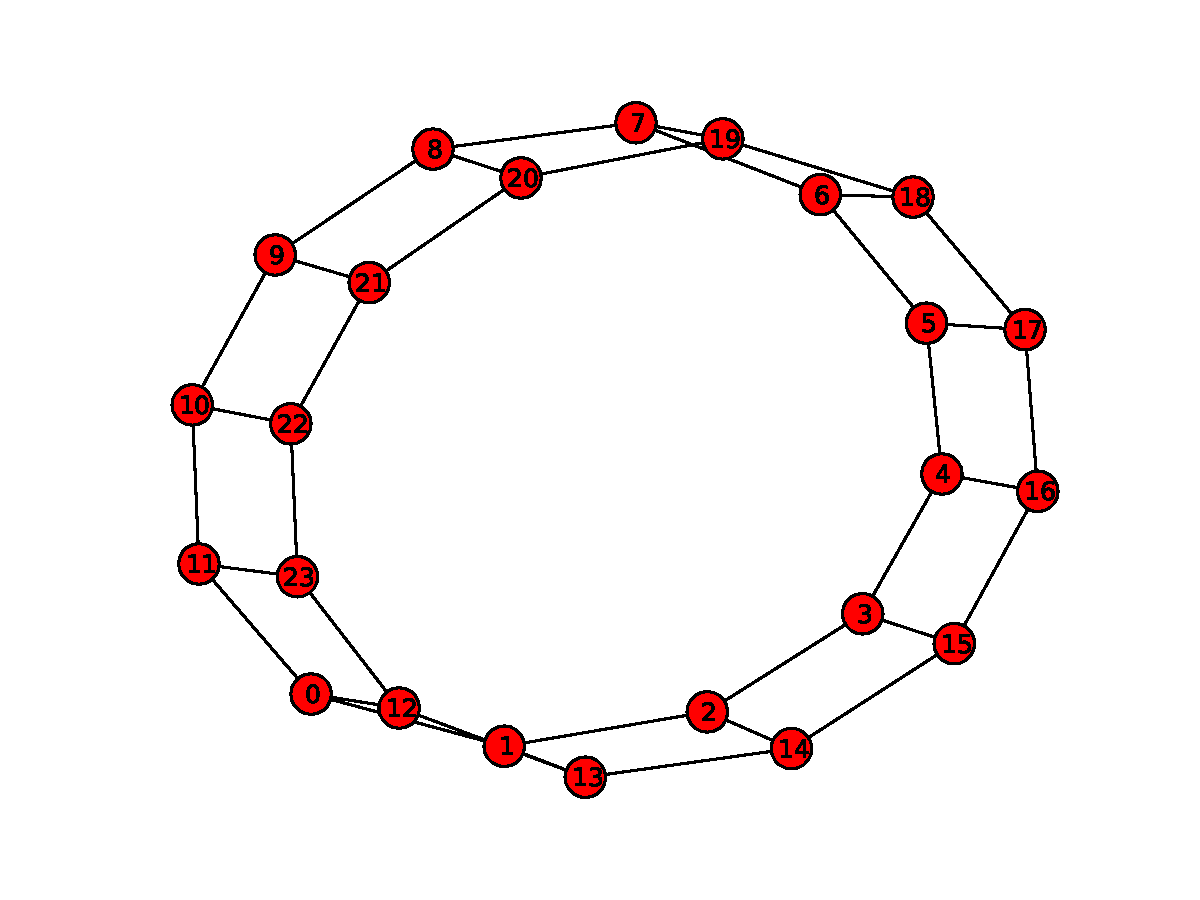
\includegraphics[width=0.7\columnwidth]{ladder}}

\end{frame}


\begin{frame}[fragile]
\frametitle{Drawing with Matplotlib}

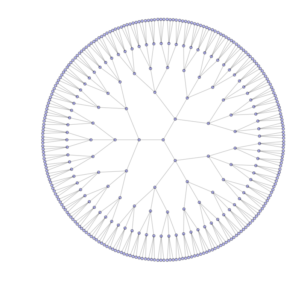
\includegraphics[width=0.25\columnwidth]{circular_tree_thumb}
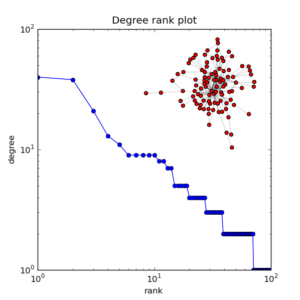
\includegraphics[width=0.25\columnwidth]{degree_histogram_thumb}
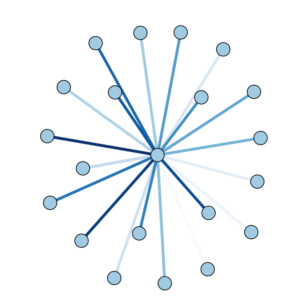
\includegraphics[width=0.25\columnwidth]{edge_colormap_thumb}
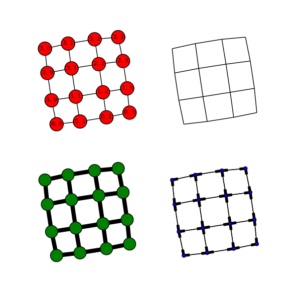
\includegraphics[width=0.25\columnwidth]{four_grids_thumb}

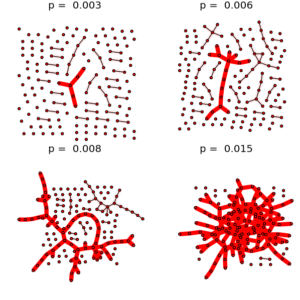
\includegraphics[width=0.25\columnwidth]{giant_component_thumb}
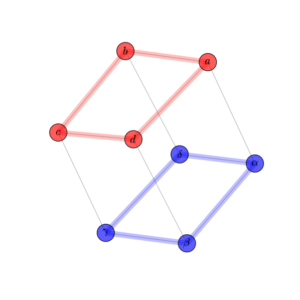
\includegraphics[width=0.25\columnwidth]{labels_and_colors_thumb}
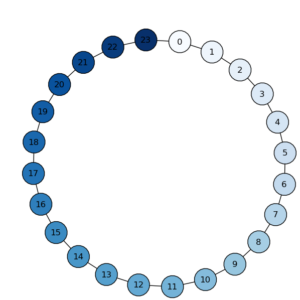
\includegraphics[width=0.25\columnwidth]{node_colormap_thumb}
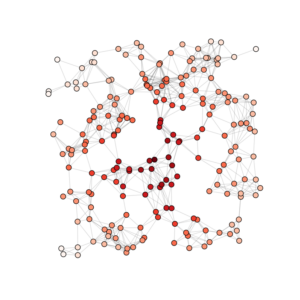
\includegraphics[width=0.25\columnwidth]{random_geometric_graph_thumb}

\end{frame}

\begin{frame}[fragile]
\frametitle{Drawing with other programs}
\centerline{Graphviz}
\centerline{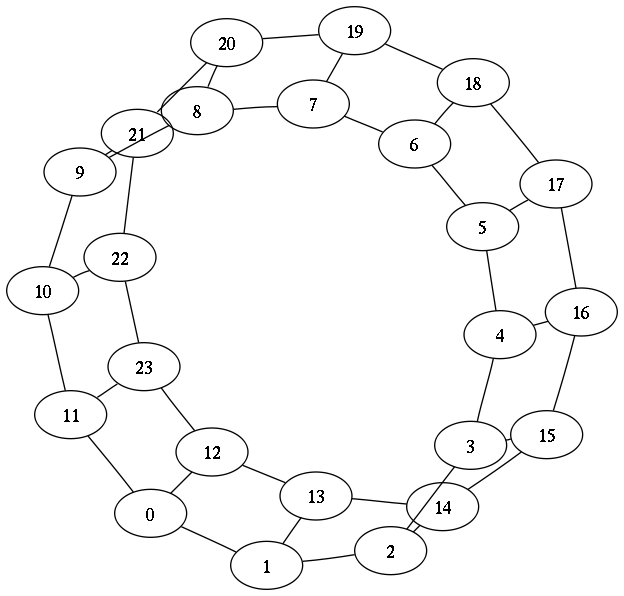
\includegraphics[width=0.5\columnwidth]{graphvizladder}}

Output to: dot, GML, LEDA, edge list, adjacency list, YAML, 
sparsegraph6, GraphML

\end{frame}


\begin{frame}
% FIXME: do a google search
\frametitle{Where is NetworkX being used?}
\centerline{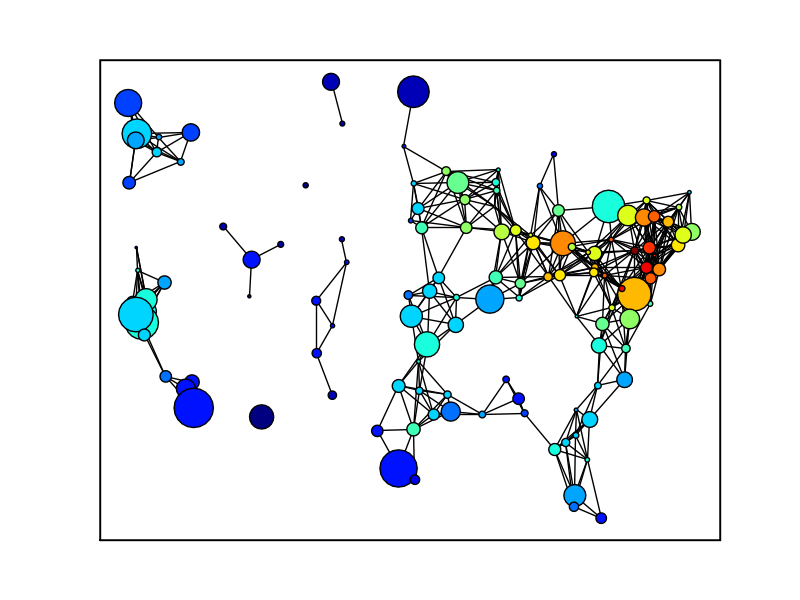
\includegraphics[width=1.0\columnwidth]{miles}}
\end{frame}


% FIXME: ``one-pager'' on sync? or interdiction, or?
%\begin{frame}
%\frametitle{Los Alamos National Laboratory: Research}
%\end{frame}


\begin{frame}
\frametitle{Los Alamos: Synchronization of networks of oscillators}

Adding red edges allows network to synchronize.

Edges found by studying network Laplacian spectrum.

\begin{figure}[ht]

\centerline{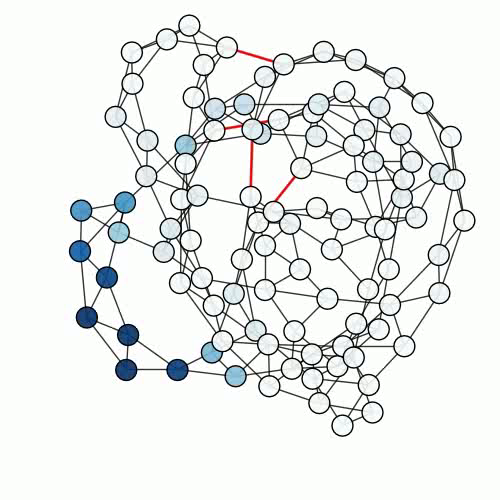
\includegraphics[scale=0.35]{sync}}
\end{figure}

{\footnotesize
Aric Hagberg and Daniel A. Schult, "Rewiring networks for
synchronization", Chaos, % vol. 18,
%\href{http://dx.doi.org/10.1063/1.2975842}{doi:10.1063/1.2975842},
%pp. 037105, 
2008 }

%{\small
%\url{http://math.lanl.gov/~hagberg/movies/sync.mp4}}
\end{frame}


\begin{frame}
\frametitle{Cornell: Education}

\centerline
INFO/SOCI 485 Computational Methods for Complex Networks  

(Gueorgi Kossinets)

Physics 7682 / Computing \& Information Sciences 6229 

(Chris Myers)

\centerline{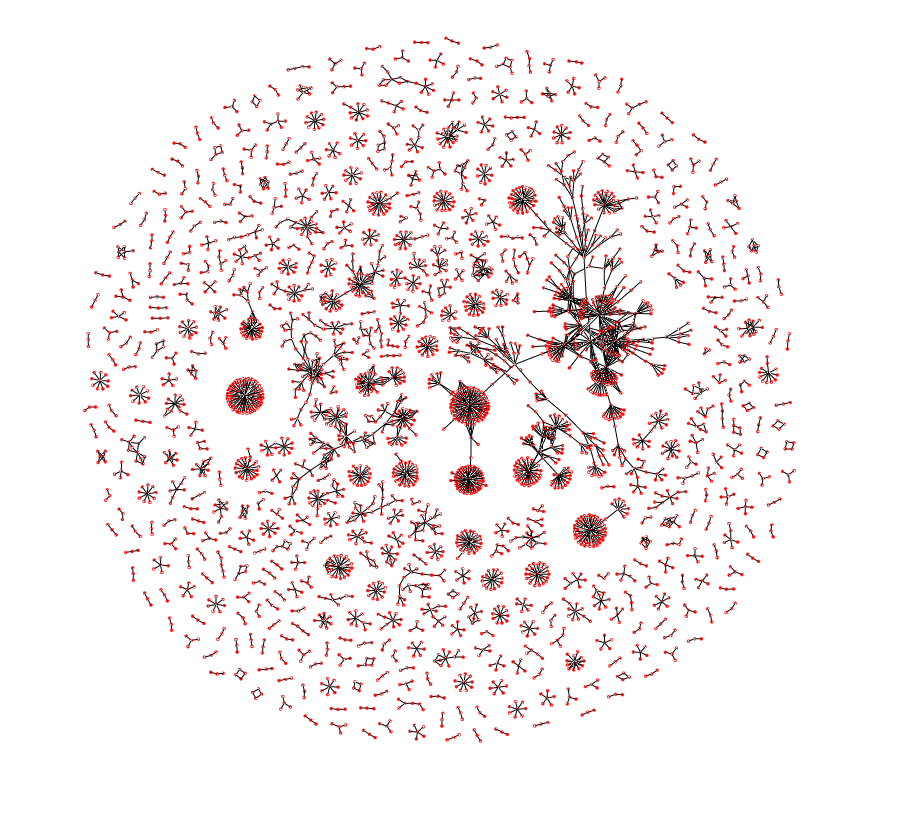
\includegraphics[width=0.7\columnwidth]{protein_pfam_net}}

\end{frame}

\begin{frame}
\frametitle{Santa Fe Institute/MIT: Data Mining}
\begin{center}
"Reality mining" (Nathan Eagle)

\centerline{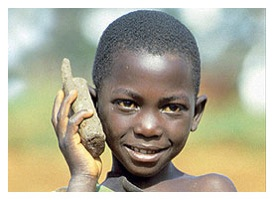
\includegraphics[width=0.5\columnwidth]{phone}}

Inferring social network structure using cell phone data 

e.g. 1.2M phone users in Rwanda
\end{center}

\end{frame}

\begin{frame}
\frametitle{FBI: Cybercrime}
\begin{columns}[c]
\begin{column}{0.1\textwidth}
\centerline{
\includegraphics[width=1.0\columnwidth]{fbi_seal}}
\end{column}
\begin{column}{0.9\textwidth}
Fighting cybercrime: botnets, spam, phishing
\end{column}
\end{columns}

\centerline{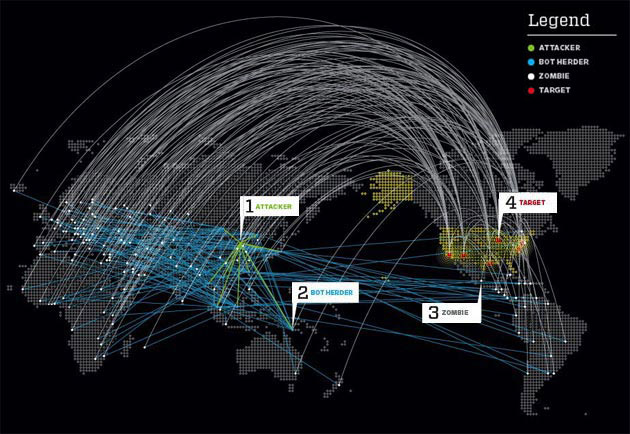
\includegraphics[width=0.9\columnwidth]{botnet}}


\end{frame}


\begin{frame}
\frametitle{Current status}

{\Large \url{http://networkx.lanl.gov/}}
\bigskip

Currently at version networkx-1.1

Active development: community driven, community supported project.

\centerline{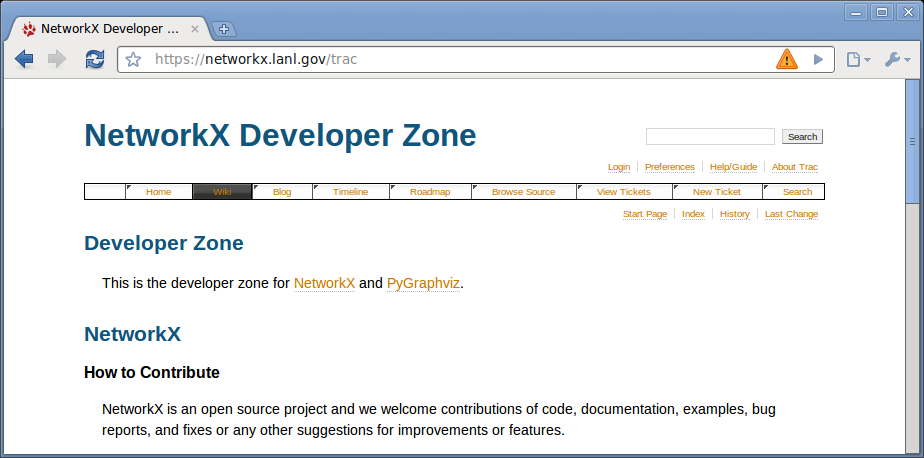
\includegraphics[width=1.0\columnwidth]{networkx-dev}}


We hope you will contribute (after class is fine).

\end{frame}



\end{document}
